\section{Globular cluster model}\label{sec:globular-cluster-model}
A globular cluster is a formation comprising a large number stars, closely packed in a spherically symmetric form \cite{britannica2024globular}.
In this work, we decided to use the implemented methods to simulate such structure using the Plummer model.
The model was chosen due to its simplicity and abundance of dedicated resources.

In the Plummer model, the density of a cluster is given by
\begin{equation}\label{eq:plummer-dens}
    \rho(r) = \frac{3M}{4\pi a^2}\left(1 + \frac{r^2}{a^2} \right)^{-5/2},
\end{equation}
where the parameter $a$ controls the spread of the distribution (the size of the cluster core) \cite{Aarseth1974Comparison}.
Hence, the particles are sampled from a distribution with PDF $p(r) = \rho(r) / M$.
Similarly to the galaxy model, we use inverse transform sampling to initialize the positions of the particles.
The marginal CDFs are easily calculated as
\begin{equation*}
    F_R(r) = \frac{r^3}{a^3}\left( 1+\frac{r^2}{a^2} \right)^{-3/2}, \quad
    F_\Theta (\theta) = \frac{1}{2}(1-\cos\theta), \quad
    F_\Phi (\phi) = \frac{\phi}{2\pi},
\end{equation*}\
which means that given a random variable $u\sim U(0, 1)$, we can generate random points with spherical coordinates
\begin{equation}\label{eq:plummer-random-init-pos}
    r = a(u^{-2/3}-1)^{-1/2}, \quad \theta = \cos^{-1}(1-2u), \quad \phi = 2\pi u,
\end{equation}
consistent with \autoref{eq:plummer-dens} (assuming equal mass of all particles).

In the Plummer model, the potential is given by
\begin{equation*}
    \phi(r) = -\frac{GM}{\sqrt{r^2 + a^2}}.
\end{equation*}
This allows us to find the escape velocity $v_e$ at distance $r$ from the center.
Using the law of conservation of energy, we get
\begin{equation*}
    \frac{1}{2}v_e + \phi(r) = 0 \Rightarrow v_e = \sqrt{-2\phi(r)}.
\end{equation*}
For any $r$, the probability distribution of $q \equiv v/v_e$ is given by \cite{Aarseth1974Comparison}
\begin{equation}\label{eq:velocity-pdf}
    g(q) = N q^2(1-q^2)^{7/2},
\end{equation}
where $N$ is a normalization constant, which can be calculated to be $N = 512 / (7\pi)$.
The CDF of the distribution in \autoref{eq:velocity-pdf}, $G(q) = \int_0^q g(q') dq'$, can be determined using symbolic integration.
The algebraic expression that one obtains in this way is lengthy and we will not cite it here.
The random values of $q$, consistent with the PDF in \autoref{eq:velocity-pdf}, are again obtained using inverse transform sampling;
the equation $G(q) = u$ is solved for $q$ by finding the roots of $G(q) - u$ using Newton's method.
Finally, the magnitude $v$ of the velocity vector $\mathbf{v}$ is set to $v = qv_e$.
The direction of $\mathbf{v} = (v_x, v_y, v_z)$ is chosen uniformly at random, i.e.
\begin{equation*}
    v_x = v\sin\theta \cos\phi, \quad v_y = v\sin\theta\sin\phi, \quad v_z = v\cos\theta,
\end{equation*}
where $\theta$ and $\phi$ are generated in the same way as in \autoref{eq:plummer-random-init-pos}.

The comparison of particle positions generated using the aforementioned method with an example of a real-world globular cluster is shown in \autoref{fig:globular-cluster-gen-vs-real}.
\begin{figure}[htp]
    \centering
    \begin{subfigure}[b]{0.4\textwidth}
        \centering
        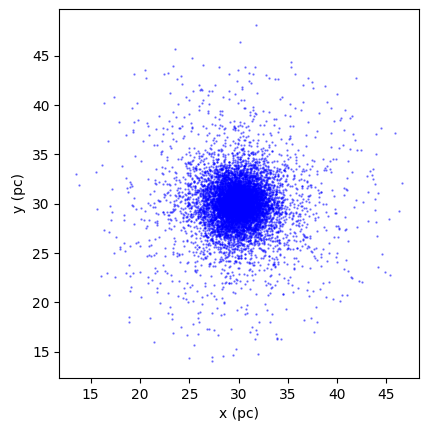
\includegraphics[width=\textwidth]{img/globular_generated.png}
        \caption{Generated data ($M=10^{6} M_\odot$, $a=2$ pc, $N=10,000$).}
        \label{fig:glob-cluster-model-generated}
    \end{subfigure}
    \hfill
    \begin{subfigure}[b]{0.4\textwidth}
        \centering
        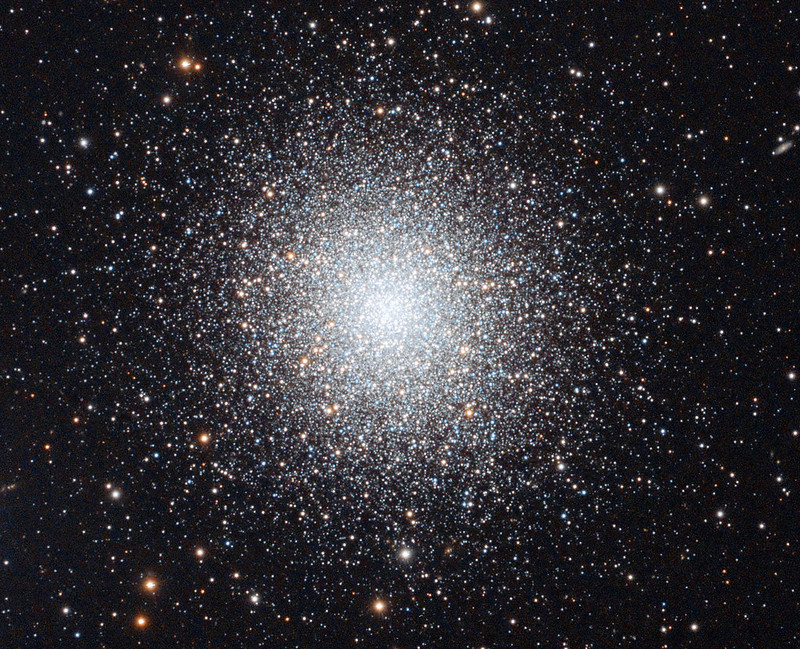
\includegraphics[width=\textwidth]{img/glob_cluster_m13.jpg}
        \caption{Real-world globular cluster (Messier 13).}
        \label{fig:messier-13}
    \end{subfigure}

    \vspace{0.5em}
    {\footnotesize
        Credit for Figure~\ref{fig:messier-13}: Giuseppe Donatiello. \par}

    \caption{The particle positions generated using the described model compared to a real-world globular cluster.}
    \label{fig:globular-cluster-gen-vs-real}
\end{figure}